\chapter{Introduction}

Anomaly detection is an important task in environments where we have a good knowledge of what is the normal behaviour but we know very little about the behaviour of anomalies. The reasons for this can be numerous: either there is no common generating principle behind the anomalies, or there is a huge disbalance in the number of labeled normal and anomalous data samples that are available for us (sometimes no anomalies are available at all), or the acquisition of anomalous data is too expensive or downright impossible (an example of this might be an industrial process). While it might be tempting to solve anomaly detection as supervised binary classification, for the reasons listed above, a supervised classificator is likely to be unrobust to actual anomalies that it will encounter in a production environment. Together with an ever-increasing volume of collected data and available computing power, this motivates the development of specialized methods for automatic anomaly detection. What these methods have in common is that they learn a model of normal data in an unsupervised manner, and detect anomalies as deviations from this model. 

Anomaly detection is important for many industries, where it is typically difficult to obtain a representative training set containing representative samples of anomalous data. The actions taken after an anomaly is detected might be varied. Sometimes, the anomaly might be considered to be an erroneous measurement and as such is ignored, which is the case of some of the earliest scientific essays~\cite{glaisher1873rejection,edgeworth1887xli} on the topic of anomaly detection. In other cases, a preventive measure must be taken in order to mitigate unwanted behaviour, such as the case of cybersecurity~\cite{liao2013intrusion, vanerio2017ensemble,xin2018machine}, fraud detection~\cite{bolton2002statistical, perols2011financial, ahmed2016survey}, medical diagnosis~\cite{tarassenko1995novelty, wong2003bayesian, iakovidis2018detecting,zhou2019anomalynet} or industrial process monitoring~\cite{mahmoudi2019layerwise, bai2020anomaly, choi2020gan}. Finally, detected anomalies might drive forward scientific discovery in astronomy~\cite{protopapas2006finding}, plasma physics~\cite{vskvara2020detection}, chemistry~\cite{oprea2002chemical} or particle physics~\cite{fraser2022challenges}.

There are countless models and algorithms for anomaly detection, tackling the problem from different angles based on the basic principle of the algorithm, the expected nature of the data and application domain. There are methods based on random forests\,\cite{liu2008isolation}, the k--nearest neighbors algorithm\,\cite{harmeling2006outliers}, Gaussian mixture models\,\cite{mahadevan2010anomaly}, clustering neural networks\,\cite{schlegl2017unsupervised}, histogram estimation\,\cite{pevny2016loda}, kernel density estimates\,\cite{latecki2007outlier} or support vector machines\,\cite{scholkopf2001estimating}. A comprehensive overview of anomaly detection methods is presented in studies such as\,\cite{pimentel2014review,goldstein2016comparative,lazarevic2003comparative,chandola2009anomaly,campos2016evaluation} where the authors compare several existing methods on benchmark datasets. Most of the comparative studies however do not include methods based
on (deep) neural networks and especially not generative models. The probably most recent and complete overview of deep generative models can be found at~\cite{ruff2020unifying}.

Deep generative models have recently attracted a lot of attention due to their ability to produce (generate) very high quality artificial images that resemble those from he training dataset. Since the seminal papers\,\cite{goodfellow2014gan,kingma2013vae,dinh2014nice} on the main types of generative models have been published, a myriad of improvements and tweaks have been proposed. While the original purpose of generative models was not aimed towards anomaly detection, some of them were redesigned for it. This text intends to collect some (but definitely not all) of the relevant information on deep generative models in one place and assess the potential suitability of the different generative models to the task of anomaly detection.

This chapter is organized in the following fashion: first, the basic principles of anomaly detection are introduced. Then we follow with a classification of anomaly detectors into main categories based on their principles and their short description, as it will be useful in the later chapters. A short section on the evaluation of anomaly detectors is followed by an overview of datasets that are frequently (and in this text) used for their experimental comparison and demonstration of their capabilities.

\section{What is anomaly detection?}
Anomaly detection has been extensively studied under many different names: outlier detection~\cite{knorr98algorithms,hodge2004survey}, novelty detection~\cite{pimentel2014review}, one-class classification~\cite{ruff2018deep} or out-of-distribution detection~\cite{liang2017enhancing}. There is a small distinction between the terms outlier, novelty and anomaly, although often times the terms are used interchangeably. The methods for their detection are however usually based on the same principle, therefore, we will resort to the use of the last term. An often cited definition of what constitutes an anomaly is ``an observation which deviates so much from other observations as to arouse suspicion that it was generated by a different mechanism''~\cite{barnett1974outliers}. This broad statement highlights the fact that anomalies may have very different sources of origin and them being anomalous depends on the context in which they are considered. 

The probabilistic definition assumes a probability distribution $P^+$ of normal data, operating on a data space $\mathcal{X}$, which is defined by a given problem, and which is most of the time known only through a set of normal samples. We can call a sample $x \in \mathcal{X}$ to be an \textbf{anomaly} if it lies in a region where $P^+$ has very low density. In other words, we can define a \textbf{set of anomalies}~\cite{ruff2020unifying} as 
\begin{equation} \label{eq:anomaly_set}
	\mathcal{A} = \lbrace x \in \mathcal{X} \vert p^+(x) \leq \tau \rbrace, \tau \geq 0,
\end{equation}
where $p^+(x)$ is the probability density function corresponding to $P^+$ and $\tau$ is a \textbf{threshold} which defines the line between normal and anomalous samples. 

It is also often assumed that the region of data space that is occupied by normal data is concentrated, that is, there exists a threshold $\tau \geq 0$ such that
\begin{equation} \label{eq:normal_concentration}
	\mathcal{X} \slash \mathcal{A} = \lbrace x \in \mathcal{X} \vert p^+(x) > \tau \rbrace
\end{equation}
is not empty, which however does not imply that the support of $p^+$ is bounded. On the other hand, $\mathcal{A}$ is not required to be concentrated and can be unbounded. Notice that we do not explicitly define any sort of anomalous distribution $P^-$. This is because most anomaly detection methods only model $P^+$. When $P^-$ is considered, such as in KDE~\cite{parzen1962estimation} or OCSVM~\cite{scholkopf2001estimating}, it is assumed that it is uniform over $\mathcal{X}$. 

\begin{figure}
\centering
\begin{subfigure}[b]{0.35\textwidth}
         \centering
         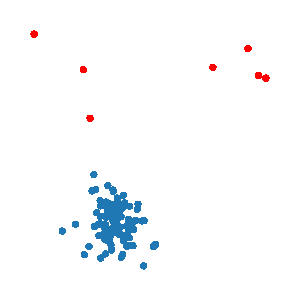
\includegraphics[width=\textwidth]{data/chapter_intro/point_anomalies.pdf}
         \caption{point anomalies}
         \label{fig:point_anomaly}
     \end{subfigure}
     \hfill
     \begin{subfigure}[b]{0.55\textwidth}
         \centering
         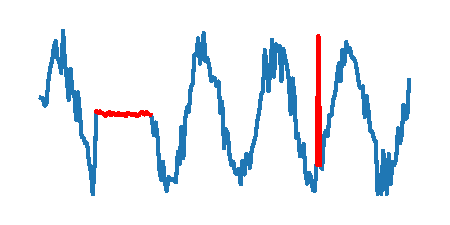
\includegraphics[width=\textwidth]{data/chapter_intro/group_anomalies.pdf}
         \caption{group (left) and contextual (right) anomaly}
         \label{fig:group_anomaly}
     \end{subfigure}

     \vspace{0.1in}

     \begin{subfigure}[b]{0.8\textwidth}
         \centering
         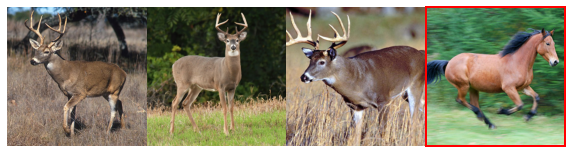
\includegraphics[width=\textwidth]{data/chapter_intro/semantic_anomalies.png}
         \caption{semantic anomaly}
         \label{fig:semantic_anomaly}
     \end{subfigure}

\caption{Examples of different types of anomalies.}
\label{fig:anomaly_examples}
\end{figure}

Different types of anomalies which require different approaches have been identified in literature~\cite{chandola2009anomaly,ruff2020unifying}. Examples are presented in Fig.~\ref{fig:anomaly_examples}.
\begin{itemize}
	\item \textbf{Point anomaly} is a single datapoint of $\mathcal{A}$, for example an outlying measurement or a photograph of a cat among other images of dogs. This is the most often studied type of anomaly in research literature. Note that a point anomaly can become an anomaly of the two following types if the datapoints in a dataset are somehow dependent (e.g. through time) or if some additional context about the data can be extracted.

	\item \textbf{Group anomalies} are a collection of correlated datapoints that are only anomalous together. Only a large number of malicious requests is enough to shut down a server in a DDoS atack~\cite{ahmed2018collective}. Other research~\cite{quellec2016multiple,wan2020weakly} focuses on finding anomalies under the multiple-instance learning (MIL)~\cite{carbonneau2018multiple} paradigm, where individual datapoints (called bags) are comprised of a variable number of observations or measurements (called instances). This calls for an aggregation method, on top of which an anomaly detector can operate.

	\item \textbf{Contextual} anomaly is a kind of anomaly that is only anomalous in certain context. A person measuring over 195~cm might be an outlier in almost any place save for a locker room of a basketball team. If a target dataset consists of pictures of birds photographed mid-flight -- is a bird sitting on grass an anomaly? Or a different flying object, such as an airplane? The answers to those questions depends on what problem is actually being solved. Contextual anomalies often arise in time series~\cite{tsay2000outliers} or in spatial data~\cite{chawla2006slom}.

	\item \textbf{Semantic} anomalies arise in image data and are opposed to \textbf{sensory} anomalies. While sensory anomalies appear in low-level image features such as edges or textures (e.g. breaks or defects), semantic anomalies can be detected in the high-level information of an image (e.g. an object of a different category than what appears in the  training dataset). Semantic anomalies can be hard to detect, as they can be very similar to normal data~\cite{ahmed2020detecting}. We will cover their detection in chapters~\ref{sec:chapter_comparison} and~\ref{sec:chapter_sgvaegan}.
\end{itemize}

We can think of any anomaly detection model as providing a function that produces ranking of the individual data points with respect to their anomalousness. This is called an \textbf{anomaly score} $s:\mathcal{X}\rightarrow\mathbb{R}$ of a model. In certain contexts~\cite{pedregosa2011scikit}, anomaly score might be called \textit{decision }or \textit{scoring function}. In this text we will assume that a higher anomaly score is attributed to a point more likely to be anomalous. As is evident from the definition, the anomaly score function does not need to be a probability in the sense of its function values lying in the interval $\left[0,1\right]$ -- in fact, some models can produce negative anomaly scores. To be able to use an anomaly score for decision making, one must choose threshold $\tau\in\mathbb{R}$. From~\eqref{eq:anomaly_set}, a sample $x$ is considered to be an anomaly if $s(x)>=\tau$ and normal otherwise. The selection of $\tau$ can sometimes be a process more complicated than the fitting of the actual model. Finally, we define the \textbf{contamination rate} of a dataset $X$, which is a finite collection of samples from $\mathcal{X}$ as
\begin{equation}\label{eq:contamination_rate}
C(\mathcal{X})=\frac{|\{x_{i}|x_{i}\in \mathcal{A} \wedge x_i \in X \}|}{|\{x_{i}|x_{i}\in X\}|},
\end{equation}
i.e. the ratio of the number of anomalies to the total size of the dataset.

\section{Comparing anomaly detectors}
Comparing different models on the same set of data is a basic requirement in practical and research problems. As already mentioned at the beginning of this chapter, anomaly detection has some common ground with binary classification tasks. For one, we can readily apply the evaluation metrics that are used to evaluate these tasks in comparisons of anomaly detectors. However, there are specifics of anomaly detection problems, mainly the often encountered large imbalance of labeled normal and anomalous samples, that we have to keep in mind. Also, with one exception, all the metrics that will be described here require at least some labeled anomalous samples, no matter how difficult it might be to obtain them.

When a sample is to be labeled as normal / anomalous, the output of the detector is compared to a threshold. Its value is typically determined on the basis of tolerated false positive rate and an estimate of the true contamination rate of a dataset~\eqref{eq:contamination_rate}.
\begin{table}
\centering
	\begin{tabular}{c | c c}
		true label/estimated label & normal & anomalous \\
		\hline
		normal & tn & fp  \\
		anomalous & fn & tp 
	\end{tabular}
	\caption{A confusion matrix of a model.}
	\label{tab:conf_ex}
\end{table}
Table~\ref{tab:conf_ex} displays the confusion table that introduces basic concepts and notation needed below. It summarizes the performance of an algorithm with a particular threshold by presenting the total number of correctly (tp = true positives and tn = true negative) and incorrectly (fp = false positives and fn = false negatives) identified samples. 

\paragraph{AUC}
The most widely used measure in the field of anomaly detection is the area under the ROC (receiver operating characteristic) curve. The acronym AUC will be used in this text for the sake of brevity). The ROC curve is a parametric curve describing the trade-off between \textbf{true positive rate} (sometimes also called \textbf{recall}) $\text{TPR}(\tau) = \frac{\text{tp}}{\text{tp+fn}}(\tau)$ and \textbf{false positive rate} $\text{FPR}(\tau) = \frac{\text{fp}}{\text{fp+tn}}(\tau)$ for different values of the decision threshold $\tau$. 

Then, the area under the curve is calculated as the following integral
\begin{equation}
\label{eq:auc}
\text{AUC}=\int_{\mathbb{R}}\text{TPR}(\tau)d\text{FPR}^{\prime}(\tau)d\tau = \int_0^1\text{TPR}(\text{FPR})d\text{FPR}.
\end{equation}
The last integral that uses $\text{TPR}(\cdot)$ as a function of the corresponding FPR shows the simple concept behind the AUC that can be easily discerned from an ROC curve drawn in a graph. An example of an ROC curve and the corresponding AUC is in Figure~\ref{fig:ROC}. In practice, the corresponding AUC is estimated from an empirical ROC curve using some numerical integration scheme, e.g. the trapezoidal rule.

As mentioned above, the main advantage of AUC is that it does not depend on the choice of a particular decision threshold. Also, the measure has a straightforward interpretation -- it is an estimate of the probability that a randomly chosen positive sample is ranked higher than a randomly chosen negative sample \cite{hand2001simple}. However a lot of information is lost when the whole ROC curve is summarized into a single number. This is especially concerning for the case of anomaly detection, where usually the region of low false positive rates is of interest, since anomalies are sparse with respect to normal data and we strive to achieve a low false positive rate. It is frequent in security applications to draw ROC curve with a logarithmic scale on the x-axis.

\begin{figure}
\centering
\begin{subfigure}[b]{0.45\textwidth} 
	\centering
	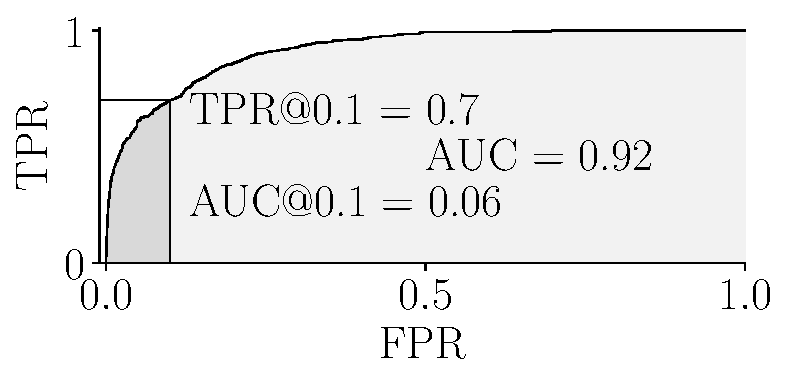
\includegraphics[width=\textwidth]{data/chapter_intro/roc_example.pdf}
	\caption{ROC curve}
	\label{fig:roc_example}
\end{subfigure}
\hfill
\begin{subfigure}[b]{0.45\textwidth}
	\centering
	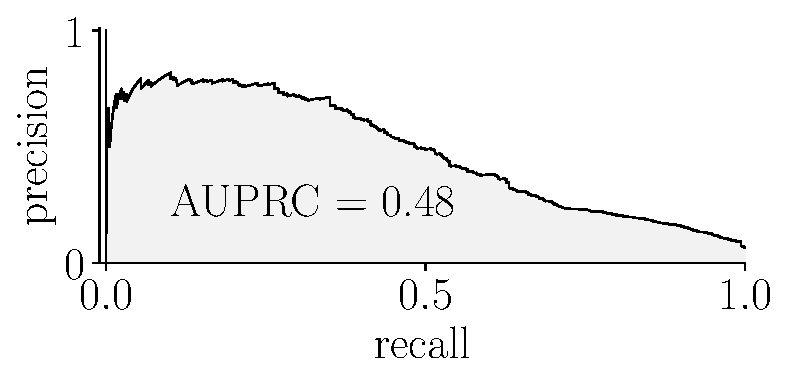
\includegraphics[width=\textwidth]{data/chapter_intro/prc_example.pdf}
	\caption{PR curve}
	 \label{fig:prc_example}
\end{subfigure}

\caption{An example of an ROC curve and the derived measures based on FPR=0.1. AUC is the whole shaded area under the ROC curve. The darker shading corresponds to AUC@0.1. On the left, the PR curve of the same detector is shown.}
\label{fig:ROC}
\end{figure}

\paragraph{AUPRC}
The Area Under the Precision--Recall Curve is very similar to AUC, as it is given by computing the \textbf{precision} $\text{PREC}(\tau)=\frac{\text{tp}}{\text{tp + fp}}(\tau)$ and recall for different values of classification threshold $\tau$ and then integrating the area under the resulting curve. A PR curve has at most as many unique recall values as positive samples in the dataset. This is problematic for anomaly detection, where the number of anomalies is low, which leads to a very sparse estimate of the true PR curve. In fact, using the same trained anomaly detector and changing the contamination rate of a testing dataset produces different AUPRC results, which then makes any analysis based on AUPRC useless when the true contamination rate is unknown. Furthermore, a correct PR curve lacks a universal starting point unlike ROC, because precision is undefined for zero recall, making the computation and normalization of the area under the PR curve and the comparison between datasets even more complicated. It is still a metric that is reported very often besides the AUC.

\paragraph{Areas of low TPR}
The two already mentioned metrics put the same weight on all areas on the x-axis. This might not be always ideal for the purposes of anomaly detection, as low FPR areas might be more interesting -- after all, when reporting detected anomalies for manual check, there is always a limit on how many samples can be realistically processed. A performance measure popular among practitioners is \textbf{\tpra}, which is simply the true positive rate (TPR) evaluated at a given false positive rate (FPR) $\alpha \in [0,1]$. This measure can be easily read from an ROC curve. In practice it is necessary to interpolate the ROC curve since FPR has discrete values, especially for datasets with a small number of samples. 

Another alternative to AUC is \textbf{\auca}, which is the area under the ROC curve calculated only up to some value of false positive rate $\alpha$. Numerically, it is important to interpolate the ROC curve for a given $\alpha$ before computing the integralIn illustration in Figure~\ref{fig:ROC}, AUC@0.1 corresponds to the darker gray region. \auca\ can be easily normalized by dividing by the chosen $\alpha$, in which case the best detector has $\auca = 1$ similarly to AUC.

\paragraph{Volume of decision region}
\begin{figure}
\centering
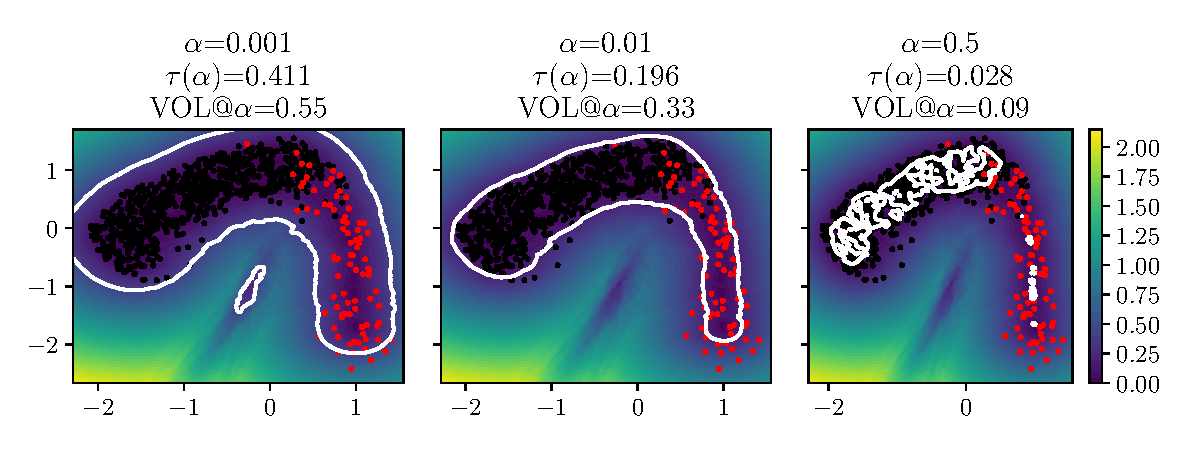
\includegraphics[scale=0.8]{data/chapter_intro/fig_vol_example.pdf}
\caption{An example of a detector and the decision region for differing values of FPR $\alpha$. The decision boundary is drawn as a white isoline at level $\tau(\alpha)$ with the estimated enclosed volume $\text{VOL@}\alpha$, black and red dots represent normal and anomalous samples in the training set. Clearly, smaller tolerance of false positives forces us to set a higher threshold which results in higher decision region volume.}
\label{fig:vol_example}
\end{figure}
All of the previous measures originate from evaluation of performance of binary detectors. Since anomaly detection is closer to one-class classification or density estimation, a measure that does not require labels for its evaluation might be more useful and better describe behaviour on unknown samples. If the goal is to compare two models supposed to characterize the normal class, it makes sense to choose the model enclosing the training data more tightly. This corresponds to calculating  the volume inside the model's decision boundary in a similar fashion to \cite{clemenccon2013scoring}, where a theoretical justification is given. This decision boundary can be chosen to correspond to a certain level of false positive rate. We define the \textbf{volume of decision region} as
\begin{equation}
  \text{VOL}(\alpha) = \int_{\mathcal{X}} \mathds{1}_{\lbrace x\in\mathcal{X}|s(x) <= \tau\rbrace} \left( x \right) dx  \text{ s.t. } \text{FPR}(\tau)=\alpha,
\end{equation}
where $\mathcal{X}$ is the input space, $s(x)$ is an anomaly score, and $\alpha$ is a given false positive rate. In other words, $\text{VOL}(\alpha)$ is the volume of subset of input space where classifier returns "normal" answer. An example of a model and its decision region for different values of $\alpha$ is shown in Fig.~\ref{fig:vol_example}. It should be noted that the idea of minizing the enclosed volume is native to some models, e.g. the OC-SVM algorithm \cite{scholkopf2001estimating}.

Computing the empirical $\text{VOL}(\alpha)$ in data space $\mathcal{X}$ is numerically estimated by Monte-Carlo methods. This comes with its downsides. Mainly, the number of samples required to cover $r$--dimensional sample space grows exponentially with $r$. This issue has been adressed in \cite{goix2016evaluate}, where the volume is computed multiple times for different subsampling of input features, however this does not seem to be optimal as it requires training a new model for each subset of features.


\section{Anomaly detectors taxonomy}

Anomaly detection methods are based on a wide range of paradigms. In this, section we will follow the taxonomy outlined in publications~\cite{pimentel2014review, ruff2020unifying}, which divide shallow (not based on neural networks) and deep (based on neural networks) detectors into groups based on their common traits. Examples of methods will be given since their knowledge will be useful in the later chapters of this text, but the list is far from complete. For a complete overview of the landscape of anomaly detection methods, see the surveys~\cite{pimentel2014review, campos2016evaluation, goldstein2016comparative, moustafa2019holistic, kwon2019survey, fernandes2019comprehensive, wang2019progress, chalapathy2019deep,ruff2020unifying}.

\subsection{Probabilistic  methods}
Since we have defined anomaly detection as detecting samples that deviate from the normal distribution $P^+$, it is straightforward to try to model the distribution by modelling its probability distribution function (pdf). One of the simplest such methods is the Grubbs' test~\cite{grubbs1969procedures}, which assumes a Gaussian distribution of the normal one-dimensional data and declares a sample to be anomalous if its distance from the mean is larger than some threshold (e.g. three standard deviations). Many such methods based on statistical tests have been proposed~\cite{barnett1994outliers}, but we will focus on advanced modelling probabilistic techniques.

\subsubsection{Shallow methods}
A \textbf{Mahalabonis distance} anomaly detector~\cite{laurikkala2000informal} builds a parametric estimate of a multivariate normal distribution by computing the mean $\mu \in \mathbb{R}^d$ and covariance matrix $\Sigma \in \mathbb{R}^{d,d}$ of the training data. The anomaly score of a test point $x \in \mathbb{R}^d$ is then
\begin{equation} \label{eq:mahalabonis_score}
	s(x) =  (x - \mu) ^T \Sigma ^{-1} (x-\mu),
\end{equation}
which is equivalent to evaluation of the negative log-likelihood under the normal distribution. Even though this is one of the simplest and most non-robust methods, terms similar to~\eqref{eq:mahalabonis_score} will be encountered a lot in the remainder of this text.

Instead of limiting the model to a single-mode distribution, a mixture of $k$ distributions 
\begin{equation} \label{eq:mixture}
	p(x) = \sum_{k=1}^K p(k) p(x|k)
\end{equation}
can be estimated instead. \textbf{Gaussian Mixture Models} (GMMs) have been used for anomaly detection in~\cite{roberts1994probabilistic,mahadevan2010anomaly}. There, we assume that $p(x|k)$ are Gaussian distribution densities and their parameters are estimated using the EM algorithm~\cite{dempster1977maximum} or via Variational Bayes~\cite{bishop2006pattern}. As the anomaly score, we can use the maximum of Mahalabonis distances~\eqref{eq:mahalabonis_score} over $k$ components. However, their use cases are limited, mainly to the need to compute and invert the covariance matrix, which is $O(d^3)$ in the size of the input space $d$.

Time series data anomaly detection was approached with the use of \textbf{Autoregressive Integrated Moving Average} (ARIMA) models in~\cite{roberts1994probabilistic,hoare2002line}, or using a \textbf{Hidden Markov Model} (HMM) in~\cite{yeung2003host,zhang2003new}. Both approaches offer predictions for future states of an observed system, and  the anomaly score is the difference between the prediction and actual state. The problems on which these methods can be applied are encountered in medicine or computer network intrusion detection.

All the previous were examples of parametric models, where a set of parameters $\theta$ is directly estimated. Opposed to these are non-parametric models, which are less restricting  -- e.g. they do not assume any (normal, Poisson, ...) distribution -- instead, they build a parameter-free model of the normal data. \textbf{Kernel density estimation} (KDE) method~\cite{parzen1962estimation}, which estimates an unknown probability density function by an empirical estimate
\begin{equation} \label{eq:kde}
	\hat{p}(x) = \frac{1}{hN} \sum_{n=1}^N k \left( \frac{x-x_n}{h} \right), x_n \in X
\end{equation}
where $X$ is the training dataset of $N$ samples, $h \in \mathbb{R}^+$ is a bandwidth parameter and $k:\mathbb{R} \rightarrow \mathbb{R}^+$ is a kernel function (uniform, triangular, normal etc.). KDE has been used under the name Parzen window estimate e.g. in~\cite{tarassenko1995novelty,yeung2002parzen}, where the $-\log \hat{p}(x)$ is used to score anomalies. \textbf{Histogram-based Outlier Score} (HBOS) is a method~\cite{goldstein2012histogram} that computes normalized histograms for each feature $x_i$ independently. Then the anomaly score for an unlabeled sample $x$ is
\begin{equation} \label{eq:hbos}
	s(x) =  -\sum_{i=1}^d \log \tilde{p}_i(x)
\end{equation}
where $\tilde{p}_i(x)$ is the height of the bin in which $x_i$ is located. The main advantage of this method in comparison with e.g. distance-based is the relative computational simplicity. In the \textbf{Lightweight Online Detector of Anomalies} (LODA)~\cite{pevny2016loda}, an ensemble of one-dimensional histograms is used in a space of diversified projection vectors. The anomaly score is then an average of the logarithm of probabilities estimated from the histograms on individual projection vectors. Due to its simplicity and computational efficiency, it is popular in settings with high volumes of data and potentially missing input values.

\subsubsection{Deep methods}
The recent advent of neural networks has given rise to many novel methods that are more capable of handling high-dimensional datasets that would be otherwise extremely difficult to handle. A mixture model was used in the \textbf{DAGMM} method~\cite{zong2018deep}, where a neural network creates a low-dimensional latent representation $z$ from an input $x$. The GMM and its parameters are then estimated in the latent space, again via a neural network, which enables online learning of the whole model together.

\textbf{Energy based models} (EBMs) use the energy function $E_{\theta}(x)$ to approximate the density as
\begin{equation} \label{eq:ebm}
	p_{\theta}(x) =  \frac{1}{Z(\theta)} \exp (- E_{\theta}(x)),
\end{equation}
where $Z(\theta)$ is the partition function to ensure proper normalization of $p_{\theta}(x)$. Although the partition function usually cannot be directly computed, an EBM can still be trained via gradient descent coupled with Markov Chain Monte Carlo estimation~\cite{hinton2002training}, which is however also the reason for its ineffectiveness relative to more novel approaches, as the MCMC is computationally costly. The anomaly score is then the energy function $E_{\theta}(x)$. Although the direct use of the early examples of EBMs such as \textbf{Deep Belief Networks}~\cite{hinton2006fast} and \textbf{Deep Boltzmann Machines}~\cite{salakhutdinov2010efficient} was impractical for anomaly detection, they were eventually refined and successfully used on anomaly detection benchmarks in~\cite{zhai2016deep}. 

Finally, the most recent advancements in anomaly detection were achieved with the use of deep generative models that model the distribution of the data via a generative process, where is is assumed that the data is generated from a hidden latent variable. \textbf{Flow models}~\cite{dinh2014nice}, \textbf{Variational autoencoders}~\cite{kingma2013vae} and \textbf{Generative Adversarial Networks}~\cite{goodfellow2014gan}  will be described in greater detail in Chapter~\ref{sec:chapter_survey}.

\subsection{Distance-based methods}
Instead of modelling the probability distribution of the normal data, distance-based anomaly detectors use heuristics that compute a well-defined similarity measure between two data points. One of the simplest such models is the \textbf{k-Nearest Neighbor} (kNN)~\cite{ramaswamy2000efficient} model where the anomaly score of a sample is based on its proximity to its $k$--nearest neighbours from the training dataset. Different proximity measures are described in~\cite{harmeling2006outliers}, where 
the Euclidean distance is used as the similarity measure and the set $X_{k}(x)$ is defined as the set of $k$-nearest neighbors of $x$ from a training dataset $X = \lbrace x_1, x_2, \ldots, x_n \rbrace \subset \mathbb{R}^d$.
\begin{itemize}
	\item $\kappa(x)$: the anomaly score is the distance between $x$ and its $k$th-nearest neighbor,
	\begin{equation} \label{eq:knn_kappa}
		s_{\kappa}(x) =  \max_{x_j \in X_k(x)} \vert \vert x - x_j \vert \vert_2,
	\end{equation}
	\item $\gamma(x)$: the anomaly score is the average distance of $x$ to its $k$-nearest neighbors, 
	\begin{equation} \label{eq:knn_gamma}
		s_{\gamma}(x) =  \frac{1}{k} \sum_{x_j \in X_k(x)} \vert \vert x - x_j \vert \vert_2,
	\end{equation}
	\item $\delta(x)$: the anomaly score is the length of the mean of the vectors pointing from $x$ to its $k$-nearest neighbours,
	\begin{equation} \label{eq:knn_delta}
		s_{\delta}(x) =  \left| \left| \frac{1}{k} \sum_{x_j \in X_k(x)} (x_j - x) \right| \right|_2.
	\end{equation}
\end{itemize}
All these definitions presume that normal data lie in concentrated regions of the data space $\mathcal{X}$, according to~\eqref{eq:normal_concentration}, while anomalies lie outside of them. The kNN anomaly detector is very popular thanks to its simplicity and performance~\cite{campos2016evaluation}. The biggest disadvantage is the computational cost. Even though there is no actual training procedure, the prediction complexity is $O(ndk)$. This can be ameliorated by the construction of a $k$-d tree~\cite{bentley1975multidimensional}, which partitions the space of the training data to speed-up prediction, or using GPU-based similarity search techniques such as~\cite{johnson2019billion}.

The \textbf{Local Outlier Factor} (LOF) algorithm~\cite{breunig2000lof} is based on comparing the local density of a sample $x$ with the local density of its $k$--nearest neighbours. To correctly describe the way in which the density is defined and the anomaly score is computed, we use the formula~\eqref{eq:knn_kappa}. Then we define the \textit{local reachability density} as 
\begin{equation}
  \text{LRD}_k(x)=\frac{|X_k(x)|}{\sum_{x_j\in X_k(x)} \max \lbrace s_{\kappa}(x), \vert \vert x - x_j \vert \vert_2 \rbrace }.
\end{equation}
Since this is basically the inverse of an average distance between $x$ and its neighbours, the closer the neighbours are to $x$, the higher this approximation of local density is. Finally, anomaly score of $x$ is given by comparing the $\text{LRD}_k(.)$ of $x$ and its neighbours 
\begin{equation}
  s_{\text{LOF}}(x)=\frac{\sum_{x_j\in X_k(x)} \text{LRD}_k(x_j)}{\text{LRD}_k(x) |X_k(x)|}.
\end{equation}
The rationale behind the formula is that if the local density of the neighbours is higher or the local density of $x$ is lower, than the more likely it is for $x$ to be an anomaly. Similar methods to LOF are the \textbf{connectivity--based outlier factor} (COF)\,\cite{tang2002enhancing} or \textbf{clustering--based local outlier factor} (CBLOF)\,\cite{he2003discovering}.

A different approach is taken by the \textbf{isolation forest }(IF) model~\cite{liu2008isolation} where an ensemble of $N_t$ isolation trees is constructed for the whole dataset. Isolation trees are constructed in such a way as to isolate each individual datapoint from the rest of the dataset using consecutive splits on different features. It is presumed that an anomaly can be isolated using a smaller number of splits and therefore it lies on a branch closer to the root of the tree. The anomaly score is then based on the number of splits of a sample averaged over multiple randomly initialized trees in the ensemble.

In \textbf{Angle-Based Outlier Detection} (ABOD)~\cite{kriegel2008angle} presumes that outliers lie far from clusters of normal data, therefore the viewing angle that covers a cluster of normal datapoints when "looking" at it from a sample $x$ is smaller when $x$ is anomalous. More concretely, the method computes the angles between $x$ and all pairs of points in the training dataset, and the anomaly score is inversely proportional to the variance of these angles -- the more varied the angles are, the more likely $x$ is close to some cluster of normal data and the anomaly score is thus lower. In the original paper, the method is lauded for the lack of hyperparameters that need to be tuned and ability to operate in high-dimensional data spaces. However, in the experiments in Chapter~\ref{sec:chapter_comparison}, it proves to be the method with one of the worst prediction times.

\subsection{Domain-based  methods}

OCSVM, SVDD, HSC

\subsubsection{Shallow methods}
In domain-based models, the data space is partitioned into subspaces by a decision boundary. Instead of estimating the density of the whole training dataset, they only consider a few samples from it, which are called \textit{support vectors}, and which are used to define the decision boundary. A very simple example is an anomaly detector which, for a training set $X = \lbrace x_1, x_2, \ldots, x_n \rbrace \subset \mathbb{R}^d$, constructs a hypersphere with center $c \in \mathbb{R}^d$ and radius $R>0$ that encloses the training data. It is found by solving the objective
\begin{alignat}{1}
\mathclap{
	\begin{aligned}
	\min_{R,c,\xi} R^2 & + \frac{1}{\nu n}\sum_{i=1}^n \xi_i \\
	\text{s.t.} \vert \vert x_i - c \vert \vert_2 & \leq R^2 + \xi_i, \xi_i \geq 0, \forall i
\end{aligned}
} \label{eq:hypersphere}
\end{alignat}
where $\xi_i$ are slack variables that allow some data points to lie outside of the hypersphere. The ratio of the maximum number outliers is controlled by the variable $\nu \in (0,1]$, which is at the same time a lower bound on the number of support vectors, which are samples $x_i$ that lie exactly on the boundary of the hypersphere. The solution to~\eqref{eq:hypersphere} is given by solving the dual problem. Notice that a simple criterion $\vert \vert x_i - c \vert \vert_2  \leq R^2$ already gives a decision whether the point $x$ is already inside the sphere. To convert this to a continuous anomaly score, we can compute the distance of $x$ from the boundary
\begin{equation}
	s(x) = \vert \vert x_i - c \vert \vert_2 - R^2
\end{equation}
which is negative for points inside and positive for points outside the hypersphere.

Abstracting the above, one can use kernel functions~\cite{shawe2004kernel} to move the problem~\eqref{eq:hypersphere} from the original input space to a transformed kernel space with higher dimension. This is the basis for the \textbf{Support Vector Data Descriptor} (SVDD) anomaly detector. By solving the problem in a space of higher dimensionality, it is possible to find a decision boundary (hypershpere) for datapoints which would otherwise not be separable in the original dimension. In comparison, the \textbf{One-Class Support Vector Machine} (OCSVM)~\cite{scholkopf2001estimating} does not construct a hypershpere, but instead aims to find a separating hyperplane in the kernel space. Unlike in traditional SVM~\cite{cortes1995support}, which is used to separate two classes in a binary classification problem, OCSVM instead aims to find a hyperplane that maximizes the separation of the majority of the training data from the origin in the kernel space. Apart from $\nu$, a very important hyperparameter of the model is the kernel scale parameter $\gamma_{\text{OCSVM}}$.

\subsubsection{Deep methods}

GT, GDAD, DSVDD, OCNN, Discriminator


\subsection{Reconstruction-based}

PCA, vQ, Kmeans?, 

AE, CAEs, DAEs, VAEs, Generator

Methods based on the \textbf{PCA }transformation\,\cite{shyu2003novel,aggarwal2015outlier}\textbf{
}are also available for anomaly detection. It is presumed that normal
data lie on a lower dimensional manifold in the data space which is
extracted by selecting the covariance matrix eigenvectors with highest
corresponding eigenvalues. The distance to this manifold is then used
as anomaly score.


\begin{figure}
\begin{centering}
\begin{tikzpicture}
  \node[const]                               (x) {$\vc{x}$};
  \node[const, right = 0.5cm of x]           (xin) {};
  % encoder in
  \node[latent, right = 0.6cm of x, yshift = 0.825cm] (E11) {};
  \node[latent, right = 0.6cm of x, yshift = 0.275cm] (E12) {};
  \node[latent, right = 0.6cm of x, yshift = -0.275cm] (E13) {};
  \node[latent, right = 0.6cm of x, yshift = -0.825cm] (E14) {};
  % encoder hidden
  \node[latent, right = 1.8cm of x, yshift = 0.55cm] (E21) {};
  \node[latent, right = 1.8cm of x, yshift = 0cm] (E22) {};
  \node[latent, right = 1.8cm of x, yshift = -0.55cm] (E23) {};
  % encoder out
  \node[latent, right = 3cm of x, yshift = 0.275cm] (E31) {};
  \node[latent, right = 3cm of x, yshift = -0.275cm] (E32) {};
  % encoder tag
  \node[const, right = 2.8cm of x, yshift = 0.825cm] (E) {$e_{\vc{\phi}}(\vc{x})$};
  % code
  \node[const, right = 4.3cm of x]           (z) {$\vc{z}$};
  \node[const, right = -0.8cm of z]           (zout) {};       
  \node[const, right = 0.5cm of z]           (zin) {};
  % decoder in
  \node[latent, right = 0.6cm of z, yshift = 0.275cm] (D11) {};
  \node[latent, right = 0.6cm of z, yshift = -0.275cm] (D12) {};
  % decoder hidden
  \node[latent, right = 1.8cm of z, yshift = 0.55cm] (D21) {};
  \node[latent, right = 1.8cm of z, yshift = 0cm] (D22) {};
  \node[latent, right = 1.8cm of z, yshift = -0.55cm] (D23) {};
  % decoder out
  \node[latent, right = 3cm of z, yshift = 0.825cm] (D31) {};
  \node[latent, right = 3cm of z, yshift = 0.275cm] (D32) {};
  \node[latent, right = 3cm of z, yshift = -0.275cm] (D33) {};
  \node[latent, right = 3cm of z, yshift = -0.825cm] (D34) {};
  % xhat
  \node[const, right = 4.3cm of z]           (xhat) {$\vc{x}'$};
  \node[const, right = -0.8cm of xhat]       (xhatout) {};       
  % decoder tag
  \node[const, right = 0.6cm of z, yshift = 0.825cm] (D) {$g_{\vc{\theta}}(\vc{z})$};
  

  % edges
  \nedge {x} {xin}
  % encoder 
  \nedge {E11, E12, E13, E14} {E21, E22, E23}
  \nedge {E21, E22, E23} {E31, E32}
  % latent
  \nedge {zout} {z}
  \nedge {z} {zin}
  % decoder
  \nedge {D11, D12} {D21, D22, D23}
  \nedge {D21, D22, D23} {D31, D32, D33, D34} 
  %xhat
  \nedge {xhatout} {xhat}

  % encoder plate
%  \plate {E} {(E11)(E14)(E32)} {};
\end{tikzpicture}

\par\end{centering}
\centering{}\caption{An example of an autoencoder consisting of fully connected layers.
The latent code $z\in\mathbb{R}^{2}$ is computed by propagating the
input $x\in\mathbb{R}^{4}$ through the encoder $e_{\phi}(x)$ and
then used to produce the reconstruction $\hat{x}\in\mathbb{R}^{4}$
via the decoder $d_{\theta}(z)$.}
\label{fig:ae}
\end{figure}

The basic idea of using an \textbf{autoencoder} (AE) for anomaly detection
is simple and was used e.g. in \cite{sakurada2014anomaly,thompson2002implicit}.
An autoencoder is a neural net that tries to propagate an input data
sample through multiple layers and produce an output that is as similar
to the input as possible. While this seems to be rather uninteresting,
the trick is that the architecture of an autoencoder is usually constrained
in such a way that the hidden layers contain less neurons than the
input and output layers, therefore preventing the autoencoder from
learning identity and forcing it to compress the data in the most
efficient way. A standard autoencoder architecture can be seen in\,\ref{fig:ae}.
It usually consists of two parts -- the decoder and encoder. Suppose
that $\mathcal{X}$ is the space of the input data and $x\in\mathcal{X}$
is an element of that space, while $\mathcal{Z}$ is the space of
samples produced by the encoder, also called the latent space. Then
we can define the encoder as a projection $e_{\phi}:\mathcal{X}\rightarrow\mathcal{Z}$
and the decoder as $d_{\theta}:\mathcal{Z}\rightarrow\mathcal{X}$.
Trainable hidden parameters (weights) of the neural network are denoted
by $\phi$ and $\theta$. Both parts of an autoencoder are trained
(the weights are adapted) using backpropagation\,\cite{werbos1982applications}
to minimize the reconstruction error with respect to $\phi$ and $\theta$

\begin{equation}
\mathcal{L}_{r}(x,\phi,\theta)=||x-d_{\theta}(e_{\phi}(x))||_{2}^{2}.\label{eq:ae_loss}
\end{equation}
The process of training and autoencoder is describe in Alg. \ref{alg:ae_train}.
Any standard optimization procedure based on gradient descent can
be used for updating in the step 6, such as the Nesterov optimizer\,\cite{nesterov1983method},
ADAM\,\cite{kingma2014adam} or AMSGrad\,\cite{reddi2019convergence}.
\begin{algorithm}

\begin{algorithmic}[1]
\Require{A training set $X=\lbrace x_j \rbrace \in \mathbb{R}^d$, maximum number of iterations $I\in\mathbb{N}$, batchsize $L \in \mathbb{N}$}
\State $\phi,\theta \gets $ Initialize parameters
\State{$i \gets $ Iteration counter}
\While{$i<I$ or $\phi,\theta$ are not converged}
	\State{$X_L \gets$ A random batch of $L$ samples from $X$}
	\State$l \gets \frac{1}{L}\sum_{j=1}^L \mathcal{L}_{r}(x_j,\phi,\theta), x_j \in X_L$
	\State$\phi,\theta \gets $ Update parameters with gradients $\nabla_{\theta,\phi} l$ to minimize $l$
	\State{$i \gets i+1$}
\EndWhile
\State{\textbf{return} encoder $e_{\phi}(x)$, decoder $d_{\theta}(z)$}
\end{algorithmic}\caption{Autoencoder training procedure}
\label{alg:ae_train}

\end{algorithm}

\begin{figure}
\begin{centering}
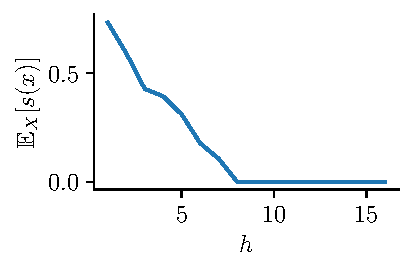
\includegraphics[scale=0.85]{data/chapter_intro/ae_reconstruction}\caption{The figure demonstrates the ability of an autoencoder to reconstruct
data. The dimensionality of the latent space $\mathcal{Z}$ is on
the x--axis, while the average reconstruction error over the whole
dataset is on the y--axis. Note that although the artificial dataset
is 16--dimensional, it only contains 8 non--correlated dimensions
while the remaining are a linear combination of them. This results
in the error dropping to zero for $\text{dim}(\mathcal{Z})>=8$ where
the model is able to disentangle the correlations and learn the identity
function.}
\label{fig:ae_reconstruction}
\par\end{centering}
\end{figure}

Suppose that $p(x)$ is the distribution of the normal data in $\mathcal{X}$
space. After training with enough examples sampled from $p(x)$, an
autoencoder should be able to reconstruct any sample from $p(x)$
almost exactly with the average error given by the constraints of
the hidden layers, as demonstrated in \ref{fig:ae_reconstruction}.
In other words, the autoencoder has learnt the shape of the distribution.
When presented with a novel sample, the ability of the autoencoder
to reconstruct it might be used to decide whether the sample comes
from $p(x)$ or not. Indeed, the most naive way of using autoencoders
for anomaly detection is assuming that $p(x)$ is the distribution
of normal data and training them using normal samples. Then, for a
novel sample $x$ the reconstruction error of the trained network
($\bar{\phi}$ and $\bar{\theta}$ are the learnt parameters of the
autoencoder)

\begin{equation}
f_{AE}(x)=\mathcal{L}_{r}(x,\bar{\phi},\bar{\theta})\label{eq:ae_score}
\end{equation}
can be used as a an anomaly score function with the assumption that
an anomaly is going to produce a larger reconstruction error due to
not coming from $p(x)$.


\subsection{Ensemble-based}

MOGAAL

\subsection{Hybrid - two-stage models}

\subsection{self-supervised methods}

\section{Anomaly detection datasets}
